\documentclass[11pt,letterpaper]{article}
\usepackage[lmargin=1in,rmargin=1in,tmargin=1in,bmargin=1in]{geometry}
\usepackage{../style/quiz}
\setbool{hideans}{true} % Student: True; Instructor: False

% -------------------
% Content
% -------------------
\begin{document}
\quiz{8}

% Problem 1
\problem If $f(x)= 5x + 8$ and $g(x)= x^2 - 4$, compute $(f \circ g)(-1)$. \par\vspace{4cm}



% Problem 2
\problem Consider the function $h(x)= 4(x + 5)^3$. Find functions $f(x)$ and $g(x)$ such that $h(x)= f \big( g(x) \big)$, i.e. write $h(x)$ as a composition of two functions. \par\vspace{4cm}



% Problem 3
\problem Compared to the graph of $f(x)$, what does the graph of $4 - f(x + 6)$ `look like'? \par\vspace{4cm}



% Problem 4
\problem Does the function $f(x)$ given below have an inverse? Explain. \par\vspace{0.2cm}

\begin{minipage}[t]{0.48\textwidth}
	\fbox{
	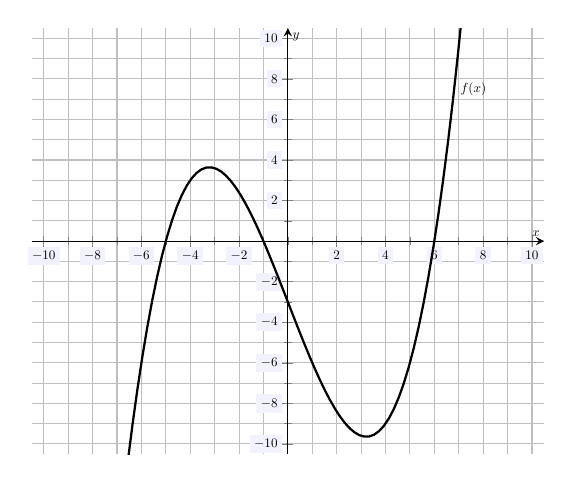
\begin{tikzpicture}[scale=0.95,every node/.style={scale=0.5}]
	\begin{axis}[
	grid=both,
	axis lines=middle,
	ticklabel style={fill=blue!5!white},
	xmin= -10.5, xmax=10.5,
	ymin= -10.5, ymax=10.5,
	xtick={-10,-8,...,10},
	ytick={-10,-8,...,10},
	minor tick = {-10,-9,...,10},
	xlabel=\(x\),ylabel=\(y\),
	]
	\node at (7.6,7.5) {$f(x)$};
	\addplot[line width= 0.03cm,samples=100,domain= -10:10] ({x},{1/10*(x+1)*(x + 5)*(x-6)});

	\end{axis}
	\end{tikzpicture}
	}
\end{minipage}

\end{document}